\chapter{Design}
\label{cha:design}
In this chapter, we motivate the design of a reactive caching system with serverless computing in Section~\ref{sec:system_goals}. In Section~\ref{sec:system_overview}, we give a general overview of our system and its building blocks, while Section~\ref{sec:system_workflow} introduces the system workflow and how those building blocks interact with each other. Chapter~\ref{cha:implementation} describes the implementation of the individual blocks in more detail.


\section{Design Goals}
\label{sec:system_goals}
Modern applications often rely on in-memory caching to improve latency-sensitive parts of their applications. Read-intensive applications can benefit significantly from in-memory caching by avoiding repeated accesses to the slow database or repeated, expensive queries of the database. Multiple distributed in-memory key-value stores, such as Memcached and Redis, are already available to provide optimized performance. In-memory caching is more expensive than slower tiers such as hard disks or SSDs, but it offers a huge performance boost, which is the main incentive for using in-memory caching. 

~\\
We first take a brief detour to Redis-based systems, which form the foundation of our in-memory caching layer and compare self-hosted Redis with ElastiCache for Redis to understand the need for a reactive in-memory caching system. We point out the current elasticity limitations regarding a fully managed service and mention the challenges of cost-effective maintenance of self-hosted Redis. This leads to the problem setting we focus on in this work and helps understand the reactive design of our system described at the end. 

\subsection{Redis-based Caching}
ElastiCache for Redis offers caching as a service within a few clicks without bothering about the actual servers underneath. The running Redis cluster is conceptually the same as a self-hosted Redis cluster on EC2 instances. However, everything ElastiCache offers is done in a few clicks, whereas with self-hosted Redis, the system administrator has to take care of it (without a simplified web interface). We mentioned an automation process that the sysadmins could use to avoid having to do this manually, but this requires a lot of effort to set up the automation process in the desired way and burdens him with much responsibility. Auto-scaling is an additional feature for ElastiCache that allows the cluster to scale as needed. The same behavior can be achieved with the automation process, only with more effort than a few clicks. Of course, the managed service comes at a price, so when comparing the hourly price, it is not surprising that the ElastiCache instance (\code{cache.t2.micro}) costs \$0.019, while the EC2 instance (\code{t2.micro}) costs \$0.0134. When comparing larger node type families, the factor even increases according to the prices on the official documentation. Another big difference is the billing granularity. While EC2 is billed per second with a minimum billing granularity of 60 seconds, ElastiCache uses a billing granularity of one hour. So as long as the cost is not an issue, ElastiCache provides a service that requires minimal system administrator effort to maintain a running and easily scalable Redis cluster. However, if cost reduction is the primary concern and the associated sysadmin effort does not get in the way, self-hosted Redis offers more customization options and finer-grained control over the Redis cluster. 

~\\
Thus, the pay-per-use model of ElastiCache is based on node hours compared to node seconds for self-hosted Redis on EC2. Depending on the billing granularity, the cost-effectiveness of the fully managed system depends heavily on the actual workload. So imagine a workload with a certain base utility and a short burst workload at the beginning of each hour that triggers ElastiCache's auto-scaling to provision an additional node for a full hour. In addition, ElastiCache is not designed for situational usage, as a cluster cannot be stopped to prevent billing if it remains unused but can only be deleted and recreated. This, combined with the billing granularity, significantly limits the cost-effective elasticity of ElastiCache for these specific workloads. 

~\\ 
On the other hand, Self-Hosted Redis is also not cost-effective in the case of burst workloads if the instance is running for the entire hour. With self-hosted Redis, the system administrator can dynamically start and stop the Redis instance to avoid paying for unused time. However, there is still some start-up time required before Redis is available. Therefore, it is difficult to set up an automation process for self-hosted Redis for burst workloads with unknown arrival times. The sysadmin either risk preemptively starting the in-memory caching layer without using it, which adds unnecessary cost, or reacting to the load, which results in poor performance because it takes time for the EC2 instance hosting the Redis server to become available. So building a cost-effective in-memory caching system in this scenario is difficult if one does not know the workload in advance. 


\subsection{Problem Setting}
The mentioned burst workloads are the primary problem setting within the scope of this work. Burst workload means only the time duration for which in-memory caching is required. For example, a burst workload of five minutes means that in-memory caching is only required for the duration of that burst, i.e., five minutes, while the rest of the time, the cache runs without being used. In the context of this work, we focus on the case where a single Redis instance can handle a load of such a burst for simplicity. The previous section has shown why providing in-memory caching for such bursty workloads can be difficult or cost-inefficient with a pure Redis-based system.

\subsection{Reactive Caching}
We address the above problems by building a reactive in-memory caching system in this work. Table~\ref{tab:layers} provides an overview of the different memory layers used in our system and their key characteristics. While self-hosted Redis is the foundation of our in-memory caching system, the main contribution of our work is the reactive design to build a cost-effective in-memory caching system and the integration of an additional in-memory caching layer in the form of serverless computing. The reactive design avoids over-provisioning of in-memory caching resources and therefore enables a cost-effective system. We emphasize the importance of responsiveness when building an in-memory caching system, as a reactive system based only on self-hosted Redis that takes a few dozen seconds to provision in-memory caching capacity is clearly suboptimal. To mitigate the long startup times of EC2 instances for self-hosted Redis, which are on the order of 30 seconds, serverless compute units are less cost-effective but available within milliseconds. The reactive design of our in-memory caching system can respond within milliseconds by leveraging the serverless platform and transitioning to the lower-cost, self-hosted Redis layer if the load persists.

\begin{table*}[t]
    \centering
    \ra{1.2}
        \begin{tabular}{ @{}l l l l l l@{} }
        \toprule
          & Layer & Latency & Startup Time & Cost & Pricing-Model \\
        \midrule
        S3 & Storage & High & - & \$ & request \& storage cost \\
        Lambda & Cache & Low & $\sim$20ms (warm-start) & \$\$\$ & billed per ms \\
         & & & $\sim$500-700ms (cold-start) & & \\
        Redis & Cache & Low & $\sim$20-50s & \$\$ & billed per second \\
        \bottomrule
        \end{tabular}
    \caption{This table shows the key characteristics of the different layers in our system. S3 is the persistent storage backend, while the in-memory caching layer includes self-hosted Redis and serverless computing.}
    \label{tab:layers}
\end{table*}

~\\
In the context of this work, we focus on the scenario of burst workloads durations less than an hour for fixed-size in-memory caching. The evaluation in Chapter~\ref{cha:evaluation} provides more details about the workload characteristics to motivate our approach, while Chapter~\ref{cha:discussion_and_outlook} discusses future work to extend our system to a fully managed scalable in-memory service similar to ElastiCache.

% Our system attempts to solve this problem by providing an additional layer of in-memory caching in the form of serverless compute units that benefit from startup times in the order of milliseconds, compared to startup times of around 30 seconds when using self-hosted Redis on EC2 instances. The additional layer is used to build a reactive system that is able to respond in time, and for the transition period where we set up a Redis cache in case the load persists. 

% \subsection{Why not just use ElastiCache?}
% % \paragraph{Amazon ElastiCache for Redis vs. Self-Hosted Redis on EC2}
% % specify differences and specifc use cases
% Building a Redis-based managed caching system raises the question of why not just use ElastiCache. This section clarifies the difference of self-hosted Redis and ElastiCache and motivates the design of our reactive caching system compared to ElastiCache.

% ~\\
% ElastiCache for Redis offers caching as a service within a few clicks without bothering about the actual servers underneath. The running Redis cluster is conceptually the same as a self-hosted Redis cluster on EC2 instances. However, everything ElastiCache offers is done in a few clicks, whereas with self-hosted Redis, the system administrator has to take care of it. We mentioned an automation process that the sysadmin can use to avoid having to do this manually, but this requires a lot of effort to set up the automation process in the desired way and burdens him with a lot of responsibility. Auto-scaling is an additional feature for ElastiCache that allows the cluster to scale as needed. The same behavior can be achieved with the automation process, only with more effort than a few clicks. Of course, the managed service comes at a price, so when comparing the hourly price, it is not surprising that the \code{cache.t2.micro} ElastiCache instance costs \$0.019, while the \code{t2.micro} EC2 instance costs \$0.0134. When comparing larger node type families, the factor even increases. Another big difference is the billing granularity. While EC2 is billed per second with a minimum billing granularity of 60 seconds, ElastiCache uses a billing granularity of one hour. So as long as cost is not an issue, ElastiCache provides a service that requires minimal system administrator effort to maintain a running and easily scalable Redis cluster. However, if cost reduction is the primary concern and the associated sysadmin effort does not get in the way, self-hosted Redis offers more customization options and finer-grained control over the Redis cluster. 

% ~\\
% Situational use of ElastiCache is difficult because the cluster cannot be stopped, only deleted and recreated. So ElastiCache doesn't really provide scaling to zero, and even if delete and recreate does the trick, ElastiCache's billing granularity still strongly discourages its use as a cost-effective situationally used cache. Self-hosted Redis, on the other hand, is a suitable building block in building a reactive in-memory caching service using serverless computing. The evaluation and discussion will further address this topic.


% This section compares the managed service ElastiCache to self-hosted Redis and explains the reference to our work. ElastiCache manages the whole server hosting and managing/monitoring which results in an easy setup within a few clicks but less flexibility with respect to the cluster configuration. Scaling takes much less effort with ElastiCache and even supports setting up auto-scaling with a few clicks, whereas with self-hosted Redis, the system administrator has to do this either manually by setting up new instances or through automation scripts, which puts a lot of responsibility and effort on the system administrator~\cite{noauthor_elasticache_nodate}. 

% When comparing prices, we consider the same node type and assume that the system overhead for the self-hosted Redis is about the same. The ElastiCache node type price for \code{cache.t2.micro} is \$0.019 per hour, while the EC2 price is \$0.0134. Without much surprise, the managed service is more expensive with a factor of 1.418. The factor for the \code{cache.r5.large} node type is 1.71 and for the \code{cache.m6g.large} node type even 1.92. Remember that Redis is mostly single-threaded (I/O handler), so using instances with multiple vCPUs does not directly increase performance as stated in the AWS documentation: you need to multiply the reported CPU usage by the number of CPU cores to get the actual usage of the single core that Redis uses~\cite{noauthor_performance_nodate}. In comparison, self-hosted Redis can easily use multiple CPUs by launching multiple instances on the same server, thus building a multi-tenant system that uses all available CPU capacity.


\section{Design Overview}
\label{sec:system_overview}
% Our system consists of several building blocks: a single orchestrator, a reverse proxy, a storage backend, and the in-memory caching layer.
This section provides a general overview of our system and its building blocks, as shown in Figure~\ref{fig:system_overview}. Clients interact with the reverse proxy to retrieve the value of a particular key. The reverse proxy acts only as a gateway, forwarding the request to the appropriate endpoint and sending back the associated response. The orchestrator manages the entire system, including the caching layer, and provides the reverse proxy with the necessary information about the corresponding endpoint. The storage backend stores key-value pairs in persistent storage, while the caching layer is responsible for high-frequency reads and consistent throughput through in-memory caching. Our in-memory caching layer consists of two building blocks based on AWS Lambda's serverless platform and the other on self-hosted Redis with EC2 instances. Although both provide in-memory capacity, the actual use case is very different due to their characteristics, as described in the previous section. The endpoint used by the reverse proxy is either the backend storage in the form of S3 or the caching layer that the orchestrator occasionally sets up. When and how our orchestrator decides to deploy an in-memory caching layer is resolved by an event-based reactive scheduler, where events contain information about recent requests in the past provided by the reverse proxy.

\begin{figure}[ht!]
    \begin{center}
        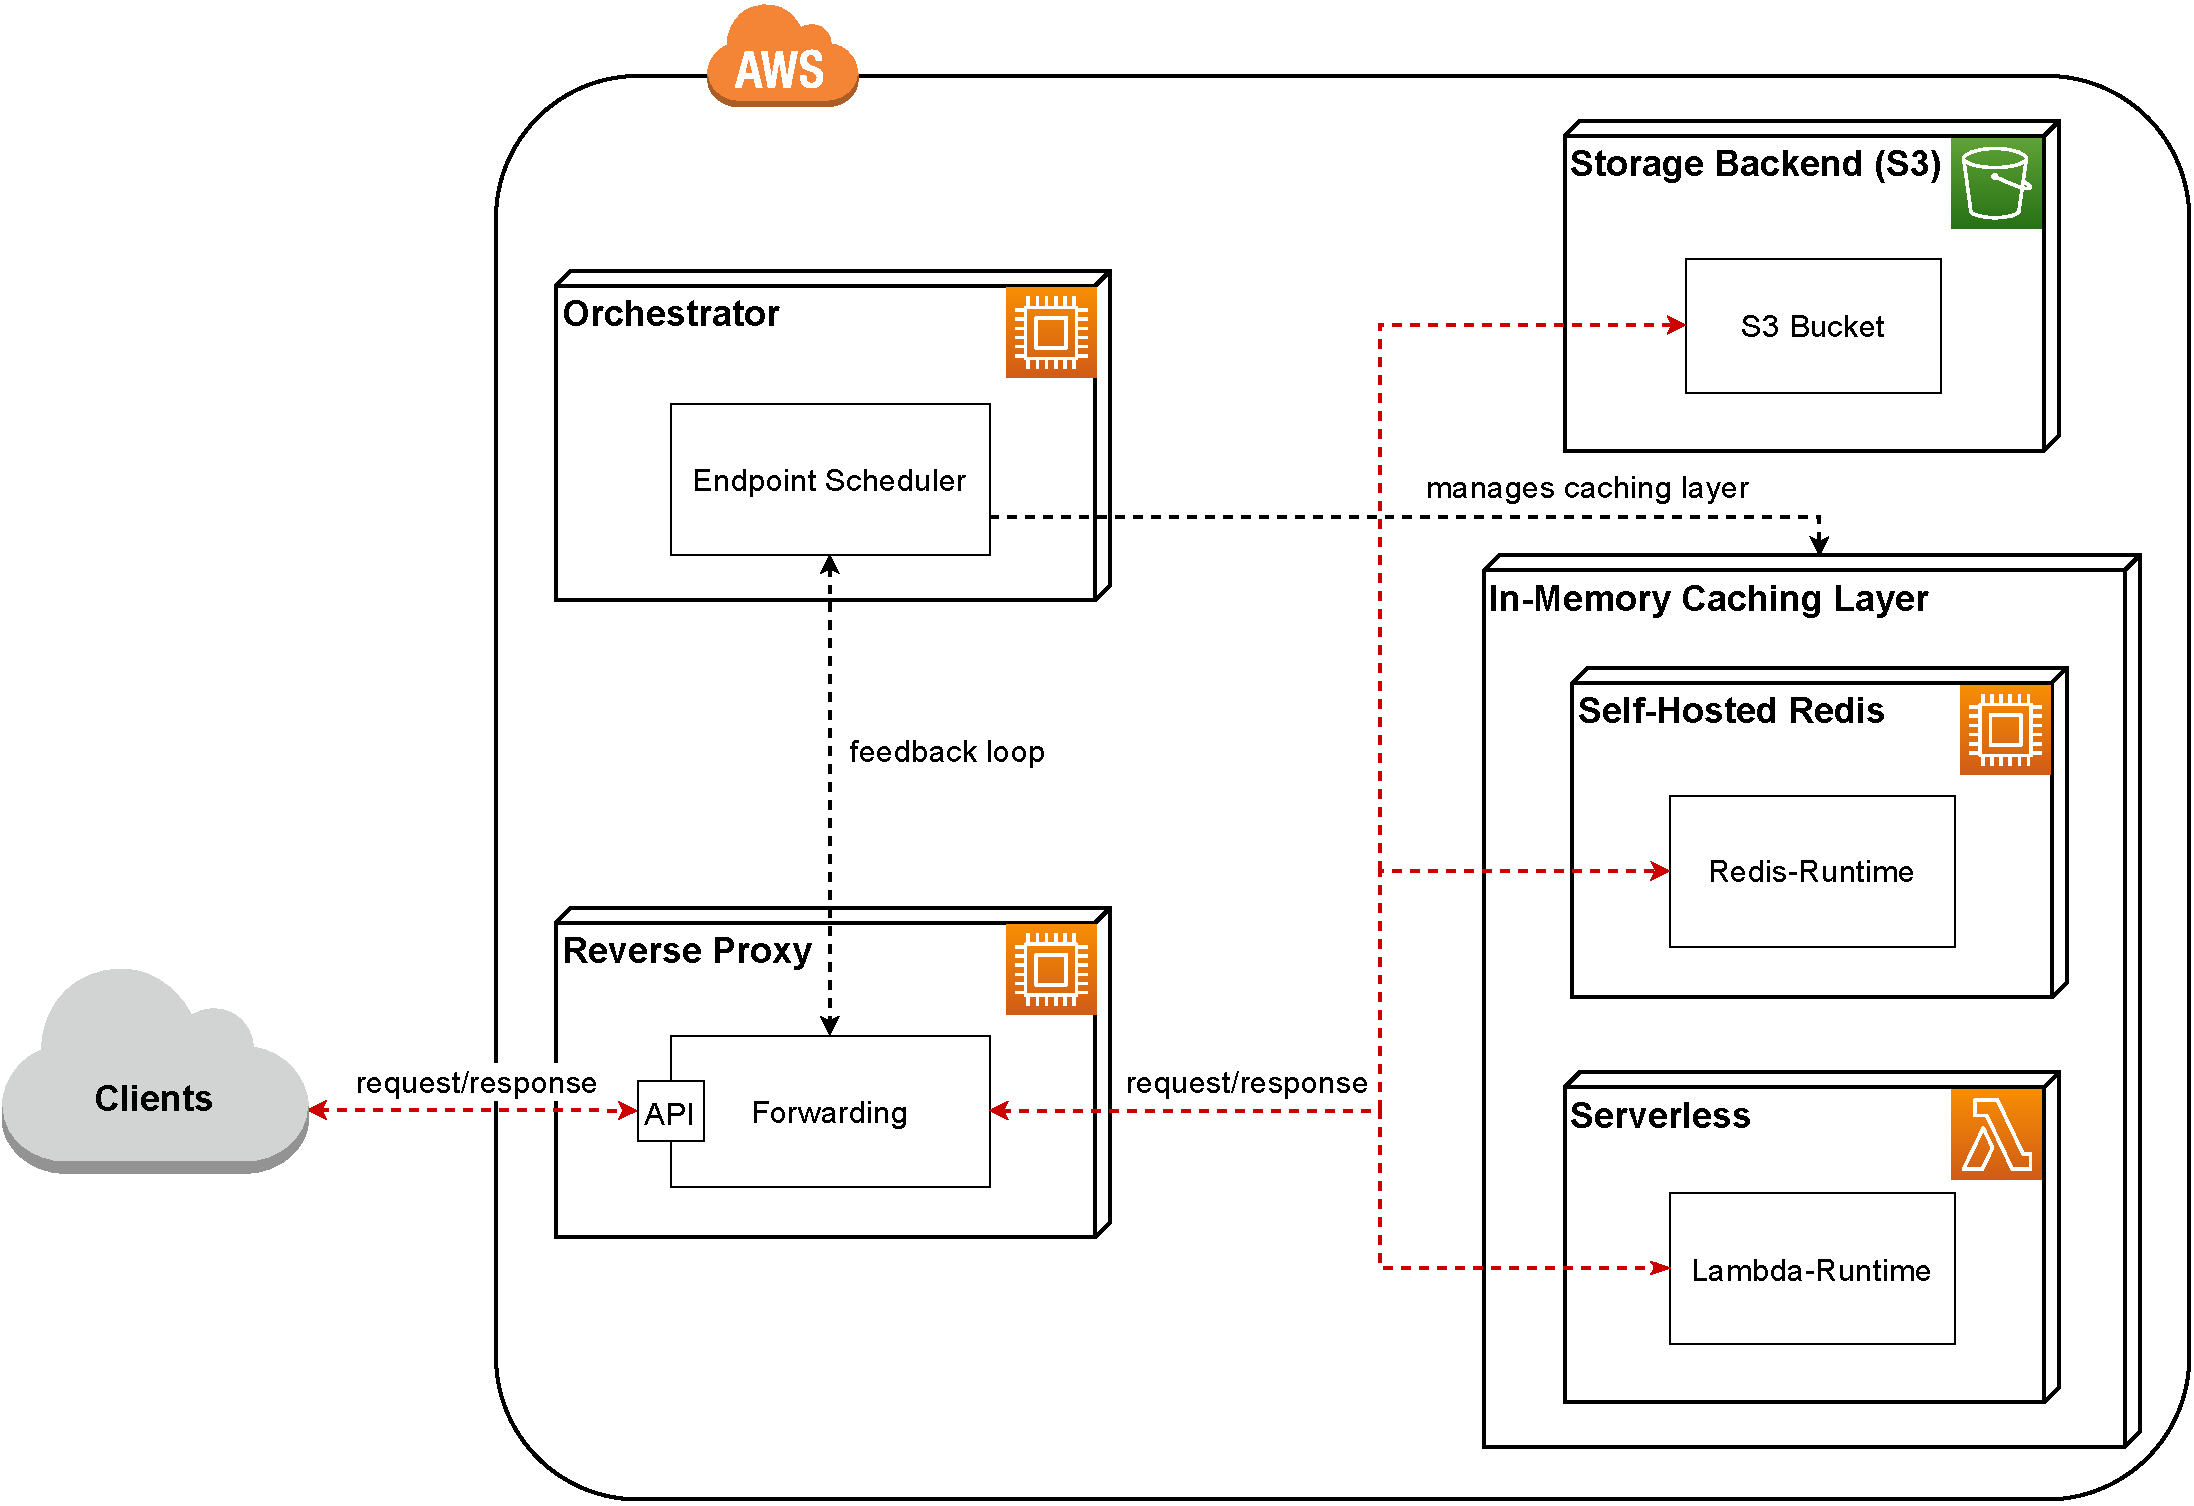
\includegraphics[width=0.95\textwidth]{figures/system_overview.pdf}
        \caption{General overview of the building blocks of our system. Only the main communication is shown, while a more detailed communication overview is given below for each individual part.}
        \label{fig:system_overview}
    \end{center}
\end{figure}

~\\
Figure~\ref{fig:system_overview} only provides a general overview of our system and the main communication channels. In Chapter~\ref{cha:implementation}, each part of the system is discussed in more detail in terms of implementation and design decisions to solve the given challenges. We also focus on how each part interacts with the others and the communication required. By deploying the orchestrator on a separate EC2 instance, we have created a system that closely adheres to the primary/secondary communication model. Therefore, our orchestrator takes on the role of the primary node that controls the other parts of the system (secondary nodes). With this design pattern, we were able to build the system in a modular fashion while maintaining a high degree of flexibility in adapting parts to changing requirements. The last point is crucial as the requirements changed and also crucial in view of Chapter~\ref{cha:discussion_and_outlook}, where we will talk about future work and the way of integrating the necessary changes into our system.

\section{System Workflow}
\label{sec:system_workflow}
This section should help to understand the workflow of our system. We describe this from the perspective of a request arriving from the client, which is the most crucial functionality since our system is built as an in-memory caching system. Also, the main contribution of our work is based on the arrival of these requests since the orchestrator that manages the whole system is a reactive event-based mechanism. This provides a good overview for the next chapter, where we describe each building block in more detail with respect to the actual implementation.

~\\
The reverse proxy does exactly what its name suggests: It accepts requests from the client and forwards the request either to the memory backend or to a running in-memory caching layer. The storage backend and self-hosted Redis are simple in that they only act as a server, while a serverless function is not intended to act as a server to which requests can be forwarded. Section~\ref{sec:serverless} will cover the serverless platform in more detail. The memory backend is always available and therefore forms the default endpoint to which our reverse proxy forwards requests, while the in-memory caching layer only runs situationally. This leads to our orchestrator, responsible for managing the in-memory caching layer and thus forms the core of our system. The reverse proxy informs the orchestrator about the requests received, which form the events that our event-based reactive orchestrator works with. Our orchestrator responds quickly and uses the serverless platform to make in-memory caching available based on these events. If the load persists with respect to these events, the orchestrator uses the serverless platform until it successfully launches the self-hosted Redis instance. Therefore, the orchestrator is also responsible for keeping the reverse proxy endpoints up to date with respect to the managed in-memory caching layers. Thus, when a new request arrives at the reverse proxy, the request is forwarded to the in-memory caching layer and not to the storage backend. 

\paragraph{Endpoint Scheduler.}
We mentioned our orchestrator's event-based, reactive design, which we will refer to as our orchestrator's endpoint scheduler. The endpoint scheduler keeps a state for each object and follows a state diagram to manage the in-memory caching layers. The endpoint scheduler changes its state and thus provides in-memory caching to the reverse proxy based on the state and events. The state diagram models the endpoint that the reverse proxy should use. The way we use serverless computing as an additional in-memory caching layer forms the first layer that provides in-memory caching. This allows our reactive endpoint scheduler to quickly respond to events that indicate a need for in-memory caching. If the demand persists, the endpoint scheduler switches to self-hosted Redis and uses the serverless platform for the startup time required by the EC2 instance hosting Redis. The instance can also be shut down again by the endpoint scheduler, and we basically start over. 
